\documentclass[14pt]{beamer}
\usepackage[utf8]{inputenc}
\usepackage[T1]{fontenc}
\usepackage{lmodern}
\usepackage[english]{babel}
\usepackage{amsmath}
\usepackage{amsfonts}
\usepackage{amssymb}
\usepackage{graphicx}
\usetheme{AnnArbor}

\newcommand\e{\emph}
\newcommand\tb{\textbf}
\newcommand\un{\underline}
\newcommand\txt{\texttt}

\AtBeginSection[]{
	\begin{frame}
	\vfill
	\centering
	\begin{beamercolorbox}[sep=8pt,center,shadow=true,rounded=true]{title}
		\usebeamerfont{title}\insertsectionhead\par%
	\end{beamercolorbox}
	\vfill
\end{frame}
}


\begin{document}
\author[Lin, J., and Graham, S.] % (optional)
{Jennifer Lin\inst{1} and Steven Graham\inst{2}}
	\title{Will God’s Grace Guide My Vote?}
	%\subtitle{}
	%\logo{}
	\institute[]{	
		\inst{1}%
		Undergraduate Student\\
		New College of Florida
		\and
		\inst{2}%
		Faculty of Psychology\\
		New College of Florida}
		
	\date[FPSA 2019]{Florida Political Science Association, March 2019}
	%\subject{New College of Florida}
	\setbeamercovered{transparent}
	\setbeamertemplate{navigation symbols}{}
	\begin{frame}[plain]
	\maketitle
\end{frame}

\begin{frame}
\begin{center}
	\e{\tb{Congress shall make no law respecting an establishment of religion, or prohibiting the free exercise thereof;} or abridging the freedom of speech, or of the press; or the right of the people peaceably to assemble, and to petition the Government for a redress of grievances} \\
	-- Amendment 1 -- Constitution of the United States
\end{center}
\end{frame}

\begin{frame}
\begin{center}
\begin{Huge}
	85\%
\end{Huge} \\
\begin{footnotesize}
	-- Putnam and Campbell, 2010
\end{footnotesize}
\end{center}
\end{frame}

\begin{frame}
\frametitle{Guiding Questions}
\begin{enumerate}
	\item Do subliminal religious primes influence political decision-making?
	\item If yes, in which direction on the left-right scale?
\end{enumerate}
\end{frame}

\begin{frame}
\frametitle{Past Research}
\begin{itemize}
	\item Religion is a central aspect to American life
	\item Personal identities shape political decision-making processes
	\item Past research suggests that individuals who vote in churches, or who are reminded of their religiosity, tend to be more conservative
	\item High costs to voting leads to a greater reliance on heuristics
\end{itemize}
\end{frame}

\begin{frame}
\frametitle{Hypotheses}
\begin{enumerate}
	\item Religious primes influence political decisions
	\item People think more conservatively in the religious mindset
\end{enumerate}
\end{frame}

\section{Experimental Method}

\begin{frame}
\frametitle{Participants}
\begin{itemize}
	\item 304 of 356 original respondents incorporated in analysis (126 identify as female)
	\item Recruited via Amazon Mechanical Turk
	\item Participants were paid \$1 for their participation
\end{itemize}
\end{frame}

\begin{frame}
\frametitle{Procedure}
\begin{itemize}
	\item Sentence Reorganization
	\item Statement and Agreement on Controversial Issue
	\item Religiosity Measure
	\item Demographic Questions
	\item Manipulation Check
\end{itemize}
\end{frame}

\begin{frame}
\frametitle{Neutral Prime}
\footnotesize
\begin{table}
	\centering
	\begin{tabular}{ll}
		\hline
		\tb{Stimuli}&\tb{Solution}\\
		\hline
		appreciated presence was imagine her&Her presence was appreciated\\
		fall was worried she always&She was always worried\\
		shoes give replace old the&Replace the old shoes\\
		retrace good have holiday a&Have a good holiday\\
		more paper it once do&Do it once more\\
		send I over it mailed&I mailed it over\\
		rode hammer he the train&He rode the train\\
		yesterday it finished track he&He finished it yesterday\\
		sky the seamless blue is&The sky is blue\\
		prepared somewhat I was retired&I was somewhat prepared\\
		\hline
	\end{tabular}
\end{table}
\end{frame}

\begin{frame}
\frametitle{Religious Prime}
\footnotesize
\begin{table}
	\centering
	\begin{tabular}{ll}
		\hline
		\tb{Stimuli}&\tb{Solution}\\
		\hline
		appreciated presence was imagine her&Her presence was appreciated\\
		his worships bent idol he&He worships his idol\\
		more paper it once do&Do it once more\\
		sacred was book refer the&The book was sacred\\
		send I over it mailed&I mailed it over\\
		the poor greed pray for&Pray for the poor\\
		yesterday it finished track he&He finished it yesterday\\
		her have in hair faith&Have faith in her\\
		prepared somewhat I was retired&I was somewhat prepared\\
		a eleven was miracle it&It was a miracle\\
		\hline
	\end{tabular}
\end{table}
\end{frame}

\begin{frame}
\frametitle{Conservative Argument}
\small
The US needs to reduce the number of women having abortions! The Government should stop supporting abortion providers like Planned Parenthood and should make abortion illegal

Here are the reasons why:
\begin{enumerate}
	\item Fetuses in the womb are unborn children – they feel pain and have the right to live
	\item	Women who have abortions often suffer physical consequences and mental anguish
	\item	It is unethical to use tax dollars to support abortion providers because so many Americans believe abortion is immoral
\end{enumerate}
\end{frame}

\begin{frame}
\frametitle{Liberal Stance}
\small
The US needs to ensure women have access to safe abortions! The Government should increase funding for abortion providers such as Planned Parenthood and should end abortion restrictions.

Here are the reasons why:
\begin{enumerate}
	\item  The government should not control women’s bodies – forcing women to bear children against their will makes them second-class citizens
	\item Making abortions illegal will result in women seeking out unsafe abortions, which are dangerous and sometimes result in death
	\item It is unfair that many women who need abortions cannot afford them. The government should find a way to reduce the cost of abortions for low-income women.
\end{enumerate}
\end{frame}

\begin{frame}
\frametitle{Religiosity Survey}
\footnotesize
\begin{center}
	\e{Each of the items here uses the following scale: 1 = Strongly Disagree to 7 = Strongly Agree}
\end{center}

\begin{enumerate}
	\item I believe the God exists
	\item Prayer to God is one of my usual practices
	\item Religion gives me a great amount of security in my life
	\item I consider myself a religious person
	\item My religion influences the way I choose to act in my routine life
	\item I feel there are more important things in life than religion
	\item I am interested in religion 
	\item Religious considerations influence my everyday affairs
\end{enumerate}
\end{frame}

\section{Results}

\begin{frame}
\frametitle{Method of Analysis}
\begin{itemize}
	\item 2 (Prime Condition) $\times$ 2 (Issue Condition) ANOVA - Between-Subjects design
	\item $\alpha = .05$
\end{itemize}
\end{frame}

\begin{frame}
\frametitle{Results}
\begin{table}
	\centering
	\small
	\begin{tabular}{lccccc}
		\hline
		\tb{Variables}&\tb{df}&\tb{SS}&\tb{MS}&\tb{F}&\tb{p-value}\\
		\hline
		Prime Condition&1&0.00&0.00&0.00&0.984\\
		Argument Condition&1&280.00&280.03&56.22&0.001***\\
		Interaction&1&0.8&0.79&0.159&0.690\\
		Residuals&288&1489.00&4.98&&\\
		\hline
	\end{tabular}\\
Note: * p$<$0.05; ** p$<$0.01; *** p$<$0.001
\end{table}
\end{frame}

\begin{frame}
\frametitle{Interaction Plot}
\begin{figure}
	\centering
	{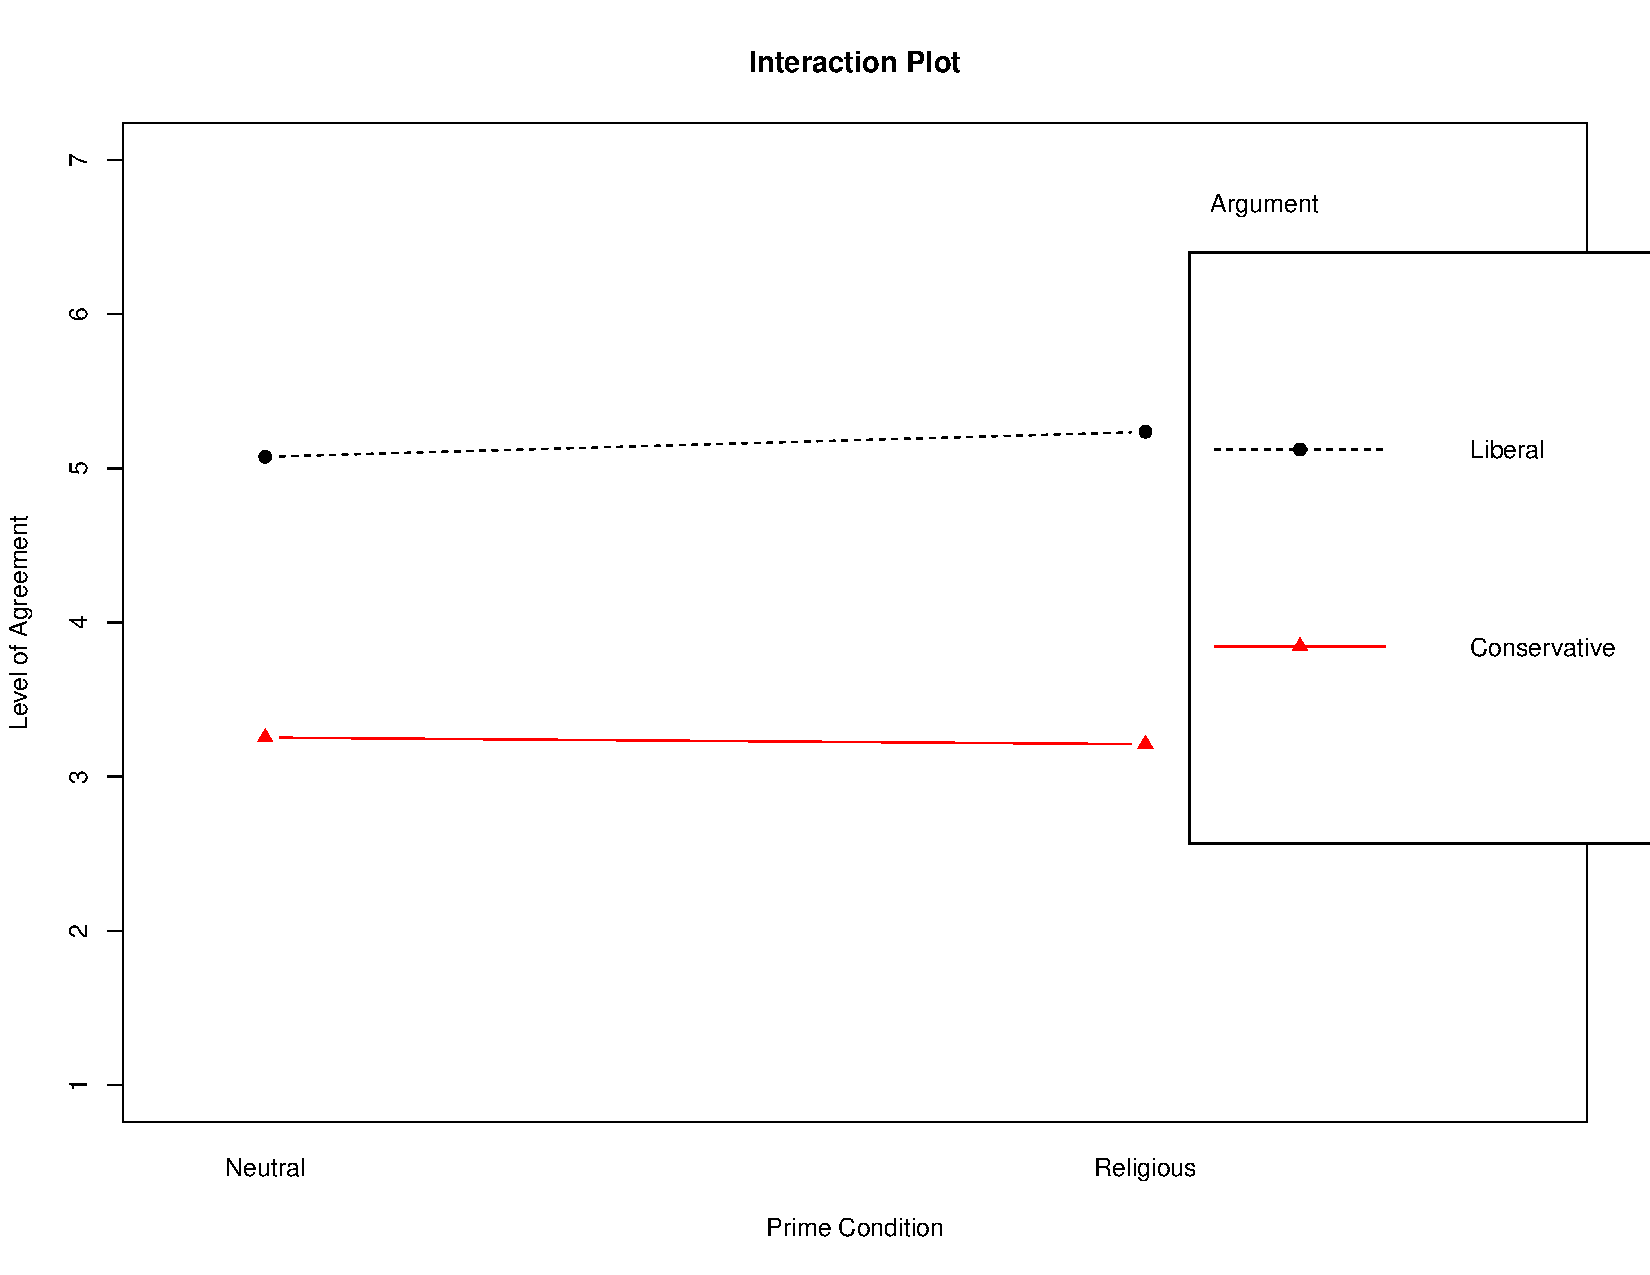
\includegraphics[width=.8\textwidth]{InteractionPlot}}
\end{figure}
\end{frame}

\section{General Discussion}

\begin{frame}
\frametitle{Conclusions}
\begin{itemize}
	\item Religious primes did not influence vote choice - No matter what priming condition participants were in, they were equally likely to voice support or reject the subject at hand
	\item Main effect present on Argument variable - Liberal position leads to greater agreement 
\end{itemize}
\end{frame}

\begin{frame}
\frametitle{Future Directions}
\begin{itemize}
	\item Limitations with Amazon Mechanical Turk and personal preconceptions
	\item Field experiment study and voter files reflecting precinct returns
	\item Use of a less polarizing subject as manipulation so that people would not enter the study with preconceived notions about the topic, which were largely reflected in their qualitative responses
\end{itemize}
\end{frame}

\section{Discussion and Questions}

\end{document}